\documentclass[twocolumn]{extarticle}
\usepackage{fontspec}   %加這個就可以設定字體
\usepackage{xeCJK}       %讓中英文字體分開設置
\usepackage{indentfirst}
\usepackage{listings}
\usepackage[newfloat]{minted}
\usepackage{float}
\usepackage{graphicx}
\usepackage{caption}
\usepackage{fancyhdr}
\usepackage{hyperref}
\usepackage{amsmath}
\usepackage{multirow}
\usepackage[dvipsnames]{xcolor}
\usepackage{graphicx}
\usepackage{tabularx}
\usepackage{booktabs}
\usepackage{caption}
\usepackage{subcaption}
\usepackage{pifont}
\usepackage{amssymb}
\usepackage{titling}

\usepackage{pdftexcmds}
\usepackage{catchfile}
\usepackage{ifluatex}
\usepackage{ifplatform}

\usepackage[breakable, listings, skins, minted]{tcolorbox}
\usepackage{etoolbox}
\setminted{fontsize=\footnotesize}
\renewtcblisting{minted}{%
    listing engine=minted,
    minted language=verilog,
    listing only,
    breakable,
    enhanced,
    minted options = {
        linenos, 
        breaklines=true, 
        breakbefore=., 
        % fontsize=\footnotesize, 
        numbersep=2mm
    },
    overlay={%
        \begin{tcbclipinterior}
            \fill[gray!25] (frame.south west) rectangle ([xshift=4mm]frame.north west);
        \end{tcbclipinterior}
    }   
}

\usepackage[
top=1.5cm,
bottom=0.75cm,
left=1.5cm,
right=1.5cm,
includehead,includefoot,
heightrounded, % to avoid spurious underfull messages
]{geometry} 

\newenvironment{code}{\captionsetup{type=listing}}{}
\SetupFloatingEnvironment{listing}{name=Code}
\usepackage[moderate]{savetrees}


\title{Computer Organization HW4}
\author{110550088 李杰穎}
\date{\today}


\setCJKmainfont{Noto Serif TC}


\ifwindows
\setmonofont[Mapping=tex-text]{Consolas}
\fi

\XeTeXlinebreaklocale "zh"             %這兩行一定要加,中文才能自動換行
\XeTeXlinebreakskip = 0pt plus 1pt     %這兩行一定要加,中文才能自動換行

\setlength{\parindent}{0em}
\setlength{\parskip}{1em}
\renewcommand{\baselinestretch}{1.25}
\setlength{\droptitle}{-7.5em}   % This is your set screw
\setlength{\columnsep}{2em}

\begin{document}

\maketitle



\section{The input fields of each pipeline register}

值得注意的是,每條 wire 後面都會標明這條 wire 是屬於哪個 stage,讓 wire 不會誤用。

\subsection{IF/ID}

\texttt{PC\_add1\_IF, instr, (instr == 0 ? 1'b0 : 1'b1)}

其中:
\begin{itemize}
\item \texttt{PC\_add1\_IF} 為 \texttt{PC+4}
\item \texttt{instr} 為 instruction
\item \texttt{(instr == 0 ? 1'b0 : 1'b1)} 為後文會提到的 \texttt{enable} 的 wire
\end{itemize}

IF/ID Register 大小為 $32+32+1 = 65$

\subsection{ID/EX}

\texttt{RegWrite\_ID, MemtoReg\_ID, Branch\_ID, MemRead\_ID, MemWrite\_ID, RegDst\_ID, ALUOp\_ID, ALUSrc\_ID, PC\_add1\_ID, ReadData1\_ID, ReadData2\_ID, sign\_ID, instr\_ID[20:16], instr\_ID[15:11], enable\_ID}

其中:
\begin{itemize}
\item \texttt{PC\_add1\_ID} 為 \texttt{PC+4}
\item \texttt{ReadData1\_ID, ReadData2\_ID} 為 register file 讀到的 \texttt{rs, rt} 資料
\item \texttt{sign\_ID} 為經過 sign extended 的 offset
\item \texttt{RegDst\_ID, ALUOp\_ID, ALUSrc\_ID} 為 EX stage 會用到的三個 control signal
\item \texttt{Branch\_ID, MemRead\_ID, MemWrite\_ID} 為 MEM stage 會用到的三個 control signal
\item \texttt{RegWrite\_ID, MemtoReg\_ID}  為 WB stage 會用到的兩個 control signal
\item \texttt{instr\_ID[20:16]} 為 \texttt{rt}
\item \texttt{instr\_ID[15:11]} 為 \texttt{rd}
\item \texttt{enable\_ID} 為後文會提到的 \texttt{enable} 的 wire
\end{itemize}

ID/EX Register 大小為 $1+2+1+1+1+2+3+1+32+32+32+32+5+5+1 = 151$

\subsection{EX/MEM}

\texttt{WB\_EX, MEM\_EX, PC\_t\_EX, zero\_EX, ALUResult\_EX, ReadData2\_EX, WriteReg\_addr\_EX, }

其中:
\begin{itemize}
\item \texttt{WB\_EX} 為 WB stage 會用到的 control signal
\item \texttt{MEM\_EX} 為 MEM stage 會用到的 control signal
\item \texttt{PC\_t\_EX} 為 branching 的 target address
\item \texttt{zero\_EX} 為 ALU 輸出 zero 的 wire
\item \texttt{ALUResult\_EX} 為 ALU 的計算結果
\item \texttt{ReadData2\_EX} 為 \texttt{rt} 的資料
\item \texttt{WriteReg\_addr\_EX} 為 WB stage 寫入的 register address
\item \texttt{enable\_EX} 為後文會提到的 \texttt{enable} 的 wire
\end{itemize}

EX/MEM Register 大小為 $3+3+32+1+32+32+5+1=109$

\subsection{MEM/WB}

\texttt{WB\_MEM, DM\_ReadData\_MEM, ALUResult\_MEM, WriteReg\_addr\_MEM, enable\_MEM}
\begin{itemize}
\item \texttt{WB\_MEM} 為 WB stage 會用到的 control signal
\item \texttt{DM\_ReadData\_MEM} 為 data memory 讀取到的資料
\item \texttt{ALUResult\_MEM} 為 ALU 的計算結果
\item \texttt{WriteReg\_addr\_MEM} 為 WB stage 寫入的 register address
\item \texttt{enable\_MEM} 為後文會提到的 \texttt{enable} 的 wire
\end{itemize}

MEM/WB Register 大小為 $3+32+32+5+1=73$

\section{Explain your control signals in sixth cycle}

我們首先看到 \autoref{fig:test1wave},可以發現在第六個 cycle 中,進到 ID stage 的 instruction 為 \texttt{0x00202816} 對應到 MIPS instruction 為 \texttt{or r5, r1, r0}。故 \texttt{RegWrite} 為 \texttt{1},代表在 WB stage 時會將資料重新寫回 register 中、 \texttt{ALU\_Op} 為 \texttt{010} 代表為 R-type 的 instruction、 \texttt{ALUSrc} 為 \texttt{0},代表 ALU 的第二個 input 為 \texttt{rt}、\texttt{RegDst} 為 \texttt{1} 代表寫入到 \texttt{rd}、\texttt{Jump, Branch, BranchType, MemWrite, MemRead} 皆為 \texttt{0},代表皆不會用到這些功能。最後 \texttt{MemtoReg} 為 \texttt{1},代表直接將 ALU 的輸出寫入到 \texttt{rd} 中。

再來看到 \autoref{fig:test2wave},在第六個 cycle 中,進到 ID stage 的 instruction 為 \texttt{0x8c020004} 對應到 MIPS instruction 為 \texttt{sw r1, 4(r0)}。故 \texttt{RegWrite} 為 \texttt{0},代表在 WB stage 時不會將資料重新寫回 register 中、 \texttt{ALU\_Op} 為 \texttt{000} 代表為 \texttt{lw},此時 ALU 可以視加法器,將 \texttt{rs} 儲存的位址加上 offset、 \texttt{ALUSrc} 為 \texttt{1},代表 ALU 的第二個 input 為 signed extend offset、、\texttt{RegDst, MemtoReg} 可以視為 don't care,因為我們不會將資料寫回到 register file、\texttt{MemWrite} 則是設為 \texttt{1},因為我們要將 \texttt{rs} 的資料透過 Data Memory 寫到 \texttt{rt+4*4} 的 address 中,最後 \texttt{Jump, Branch, BranchType, MemRead} 皆為 \texttt{0},代表皆不會用到這些功能。


\begin{figure}[H]
\centering
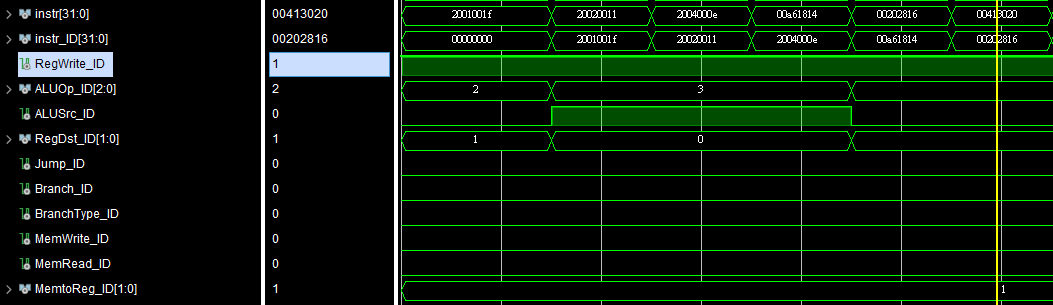
\includegraphics[width=\linewidth]{test1_wave}
\caption{CO\_P5\_test\_data2 之波形圖,圖中黃色線所在的 cycle 為第六個 cycle}
\label{fig:test1wave}
\end{figure}

\begin{figure}[H]
\centering
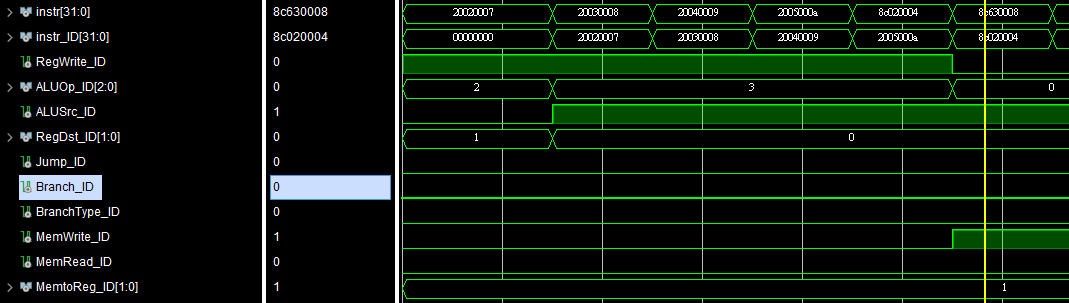
\includegraphics[width=\linewidth]{test2_wave}
\caption{CO\_P5\_test\_data1 之波形圖,圖中黃色線所在的 cycle 為第六個 cycle}
\label{fig:test2wave}
\end{figure}


\section{Problems you met and solutions}

當第一個指令仍在 IF stage,因為 pipeline register 的預設值皆為 0,故在第一個 cycle 中,ID stage 會 decode \texttt{0x00000000} 這個 instruction,這個 instruction 會被我的 decoder decode 為 \texttt{sll r0, r0, 0} 而且因為在 HW4 中,原本的架構有 shifter 和 zero\_filled 的設計,所以有一個 \texttt{FURslt} 的 MUX,所以 sll 的 \texttt{ALU\_operation} 我並沒有認真設計,而是直接打為 \texttt{1000},故最後 \texttt{ALU} 算出的結果會是 \texttt{$\sim$r0 or r0} = \texttt{0xffffffff},且這個結果會被存回去 \texttt{r0} 中,導致後面的計算發生錯誤,為了解決這個問題,我後來的解法是在每個 pipeline register 中加入 \texttt{enable} 這個 wire,當資料在 data memory 或是 register file 寫入時,會去跟 \texttt{enable} AND,如果 \texttt{enable} 是 1 時,資料才有可能寫入,而這個值是在 IF stage 中檢查目前進來的 instruction 是不是 \texttt{0x00000000} 決定的,如果是 \texttt{0x00000000},則這個值會設為 0,代表計算結果不會寫入到 memory 中。經過以上的操作後,結果就會是正確的。

\section{Summary}

在本次作業中,我了解如何設計 Pipeline Register,並透過在 Single Cycle CPU 中加入 Pipeline Register 達到 Pipeline 的效果。也透過接線的過程,了解 CPU 中會需要哪些 control signal,各個 control signal 是在哪個 stage 被用到。在這次作業中,更加了解 CPU 整個 data flow 的流程。

\end{document}